\documentclass{article}


\usepackage[margin=0.6in]{geometry}
\usepackage{amssymb, amsmath, amsfonts}
\usepackage{tabularx}
\usepackage{arydshln}
\usepackage{mathtools}
\usepackage{changepage}
\usepackage{asymptote}
\usepackage{cancel}
\usepackage{physics}
\usepackage{pgf}
\usepackage{enumerate}
\usepackage{placeins}
\usepackage{nth}
\usepackage{array}
\usepackage{tikz}
\usetikzlibrary{arrows,automata}
\tikzset{
  saveuse path/.code 2 args={
    \pgfkeysalso{#1/.style={insert path={#2}}}%
    \global\expandafter\let\csname pgfk@\pgfkeyscurrentpath/.@cmd\expandafter\endcsname
      % not optimal as it is now global through out the document
                           \csname pgfk@\pgfkeyscurrentpath/.@cmd\endcsname
    \pgfkeysalso{#1}},
  /pgf/math set seed/.code=\pgfmathsetseed{#1}}
\usepackage{nicefrac}
\usepackage{pgfplots}
\usepgfplotslibrary{polar}
\pgfplotsset{holdot/.style={fill=white,only marks,mark=*}}
\pgfplotsset{soldot/.style={only marks,mark=*}}
\newcommand{\enth}{$n$th}
\newcommand{\Rl}{\mathbb{R}}
\newcommand{\Cx}{\mathbb{C}}
\newcommand{\sgn}[1]{\text{sgn}\qty[#1]}
\newcommand{\ran}[1]{\text{ran}\qty[#1]}
\newcommand{\E}{\varepsilon}
\newcommand{\qiq}{\qquad \implies \qquad}
\newcommand{\half}{\nicefrac{1}{2}}
\newcommand{\third}{\nicefrac{1}{3}}
\newcommand{\quarter}{\nicefrac{1}{4}}
\newcommand{\f}[3]{#1\ :\ #2 \rightarrow #3}
\newcommand{\Dx}{\Delta x}
\newcommand{\Dy}{\Delta y}
\newcommand{\Dt}{\Delta t}
\newcommand{\hot}{\text{h.o.t.}}
\newcommand{\centdiff}{\frac{u_j^{n+1} - u_j^n}{\Dt}}
\newcommand{\dod}{Domain of Depdendence}

\newcommand{\tridsym}[3]{
    \qty(\begin{array}{ccccc}
                    #1 & #2 & & & \\
                    #3 & #1 & #2 & & \\
                    & \ddots & \ddots & \ddots &  \\
                    & & #3 & #1 & #2 \\
                    & & & #3 & #1
                \end{array})
}


\DeclareMathOperator*{\esssup}{\text{ess~sup}}

\title{MAT 228B Notes}
\author{Sam Fleischer}
\date{March 3, 2017}

\begin{document}
    \maketitle

    The Modifed equation for Lax Windroff is
    \begin{align*}
        v_t + a v_x = \mu v_{xxx} \qquad \qquad \text{where } \mu = \frac{a\Dx^2}{b}\qty(\nu^2 - 1)
    \end{align*}
    The solution to the PDE is
    \begin{align*}
        v(x,t) = \frac{1}{\sqrt{2\pi}}\int_{\mathbb{R}}\hat{v}(\xi,0)e^{-i\xi(x - c(\xi)t)}\dd\xi \qquad\qquad \text{where } c(\xi) = a + \mu\xi^2
    \end{align*}
    The wave will travel at constant speed $c$, not constant speed $a$.  $c(\xi)$ is known as the phase velocity.  Low spatial frequency data ($\xi$ small) travels at about the correct speed (close to $a$).  High spatial frequency data ($\xi$ large) travels at a notably different speed than $a$.

    What is the difference in diffusion and dispersion.  Diffusion is high frequencies getting damped.  Dispersion is high frequencies moving away fast.

    Why is dispersion so much worse for discontinuous initial conditions?  There is a large amount of high frequencies.  For $u$ piecewise smooth with jump discontinuities, then $\hat{u}(\xi)$ scales like $\frac{1}{\abs{\xi}}$ for large $\xi$.  If $u$ is $C^\infty$, then $\hat{u}(\xi) = \order{\frac{1}{\abs{\xi}^p}}$ for any $p$.  For example, $C^\infty$ and some other condition, $\hat{u}(\xi)$ decays like $e^{-a\abs{\xi}}$.

    We could include more terms and get a better modified equation though..
    \begin{align*}
        v_t + av+x = \mu v_{xxx} - \E v_{xxxx}
    \end{align*}
    where $\E = \order{\Dx^3}$.  Now, Lax-Windroff gives 4th order accurate solutions to this equation.  The fourth order is dissipative... it damps high frequencies faster than diffusion and it damps low frequencies slower.

    \section{Convergence Analysis of Upwinding on Discontinuous Initial Data}

        We have
        \begin{gather*}
            u_t + au_x = 0 \\
            u(x,0) = u_0(x) = \begin{cases}
                1 & x \leq 0 \\
                0 & x > 0
            \end{cases}
        \end{gather*}
        The solution is $u(x,t) = u_0(x - at)$.  If we had $v_t + av_x = Du_{xx}$ with $v(x,0) = u_0(x)$, upwinding gives second-oreder accuracy.  How accurately does $v$ capture the behavior of $u$?  The solution is $v(x,t) = 1 - \erf(\frac{x - at}{\sqrt{4Dt}})$.  The error function $\erf$ is
        \begin{align*}
            \erf(x) = \frac{2}{\sqrt{\pi}}\int_{-\infty}^x e^{-z^2}\dd z
        \end{align*}
        The length scale is $\sqrt{4Dt}$.
        \begin{figure}[ht!]
            \centering
            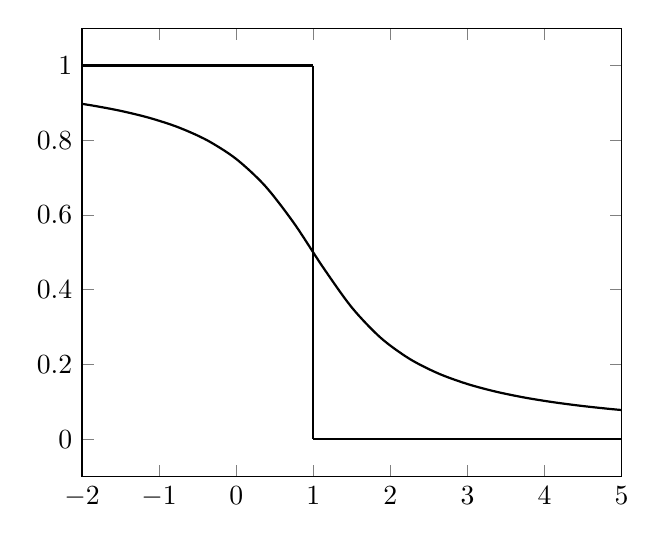
\begin{tikzpicture}
                \begin{axis}[xmin=-2,xmax=5]
                    \addplot[domain=-3:1,thick] {1};
                    \addplot[domain=1:6,thick] {0};
                    \addplot[domain=-3:6,smooth,thick] {-1/180*atan(x-1)+0.5};
                    \draw[thick] (axis cs:1,1) -- (axis cs:1,0);
                \end{axis}
            \end{tikzpicture}
        \end{figure}
        \FloatBarrier
        So upwinding does not converge in $\infty$-norm for a discontinuous problem.  Convergence in $1$-norm:
        \begin{align*}
            \norm{u - v}_1 = \int_{\mathbb{R}}\abs{u(x,t) - v(x,t)}\dd x = \int_{\mathbb{R}}\abs{u_0(x - at) - \qty(a - \erf(\frac{x - at}{\sqrt{4Dt}}))}\dd x
        \end{align*}
        Letting $z \coloneqq x = at$, 
        \begin{align*}
            \norm{u - v}_1 = \int_{-\infty}^0\erf(\frac{z}{\sqrt{4Dt}})\dd z + \int_0^\infty 1 - \erf(\frac{z}{\sqrt{4Dt}})\dd z = 2\int_{-\infty}^0\erf(\frac{z}{\sqrt{4Dt}})\dd x
        \end{align*}
        Now letting $s \coloneqq 2\sqrt{4Dt}\int_{-\infty}^0\erf(s)\dd s$,
        \begin{align*}
            \norm{u - v}_1 = 2\sqrt{4Dt}\int_{-\infty}^0\erf(s)\dd s.
        \end{align*}
        So, for upwinding, if $D = \order{\Dx}$, $\norm{u - v}_1 = \order{\sqrt{\Dx}}$.  Upwinding converges at order $\frac{1}{2}$ in the 1-norm for discontinuous initial data.

\end{document}












